%!TEX root = ../main.tex

\chapter{\texorpdfstring{Precision \nnbb\ distribution analysis}{Precision 2νββ distribution analysis}}%
\label{chap:2nbb-ana}

As extensively demonstrated in \cref{chap:theory}, the \nnbb\ event distribution is of
great interest for new-physics searches. Many of these exotic processes can indeed
generate distortions in the energy spectrum shape predicted by the Standard Model. The
most frequently-considered phenomena, namely neutrinoless double-beta decay with Majoron
emission (\onbbx, \onbbxx) and Lorentz-violating two-neutrino double-beta decay (\nnbblv)
have been reviewed in \cref{chap:theory}. The aim of the research presented in this
chapter is to constrain the presence of these distortions in the \nnbb\ events collected
by \gerda\ in the first part of \phasetwo, by setting limits on the theoretical model
parameters that regulate their magnitude. Moreover, a new estimate of the \nnbb\ half-life
\thalftwo\ will be presented with a reduced systematic uncertainty compared to past
publications~\cite{Agostini2015a}. To improve the sensitivity of the analysis the data
after the liquid argon veto cut is considered for the first time. As already shown in
\cref{sec:bkg:lar:ph2:gmodel}, in fact, the signal-to-background ratio improves by a factor of 10
in the \nnbb\ energy region after the cut. Furthermore, to reduce the systematic
uncertainties connected to the detector active volume model, data from enriched
semi-coaxial detectors is discarded. The low background level (signal-to-background ratio
of $\sim$20 in the \nnbb\ region excluding the potassium \g\ lines) and the high-statistic
signal data sample ($\sim$$5 \cdot 10^{4}$~\nnbb\ events above the \Arl\ Q-value,
see \cref{tab:bkg:lar:ph2:results}) motivates the construction of a high-precision fit
of the \nnbb\ energy distribution to test the validity of the Standard Model predictions.
\newpar
This chapter is divided in three sections: the data selection and the statistical methods
which are used to study the signal sensitivity and analyze the data set are presented in
\cref{sec:2nbb-ana:stat}, while sources of systematic uncertainties and their effect on
the analysis are extensively described in \cref{sec:2nbb-ana:systematics}. The
results are finally presented and discussed in \cref{sec:2nbb-ana:results}.

\section{Statistical analysis}%
\label{sec:2nbb-ana:stat}

\blocktitle{data and \\ pdfs}
The \enrBEGeII\ data set after the LAr veto cut (already characterized in
\cref{sec:bkg:lar:ph2:data}, see \cref{fig:bkg:lar:ph2:data-desc} (top panel) for the
energy spectrum) has been considered for this analysis both because of the higher
signal-to-background ratio in the \nnbb\ region of about 20 (excluding the two potassium
\g\ lines) compared to data before analysis cuts and for the lower uncertainty in the
\bege\ detectors active volume determination (see \cref{apdx:gedetav}).
\newpar
The theoretical predictions for signal and background event distributions are obtained, as
usual, from Monte Carlo simulations through the \mage\ software framework. The LAr veto
model, which is extensively described in \cref{sec:bkg:lar:ph2:pdfs}, is used to compute
the LAr veto flag for synthetic events. A selection of pdfs is shown in
\cref{fig:bkg:lar:ph2:pdfs:gmodel}. The same pdf sample considered in the background model
after the LAr veto cut (\cref{sec:bkg:lar:ph2:gmodel}) has been selected to represent the
background in this analysis. The choice of a reduced set, compared to the background model
before analysis cuts, is motivated by the fact that the description of the shape of such a
low background does not benefit from more complex models, from the statistical point of
view. The obtained goodness-of-fit for the \enrBEGeII\ data set in the \nnbb\ region is,
indeed, satisfactory enough (see \cref{fig:bkg:lar:ph2:results-closeup}), and the
impact of different pdf shapes (e.g.~\Ac\ far or close to the detector array) is assessed
in the analysis of the systematic uncertainties. Note that the information from the
\enrCoaxII\ and \enrGeII\ data sets is also missing.
\newpar
The likelihood function defined to compare data and expectations is the usual Poisson
likelihood which runs over the binned \enrBEGeII\ energy spectrum:
\[
  \mathcal{L}(S, \vec{B} | \vec{n}) =
    \prod_i^{N} \frac{{\nu_i(S, \vec{B})}^{n_i} e^{\nu_i(S, \vec{B})}}{n_i!} \;,
\]
where $i$ is the bin index, $N$ is the number of bins, $n_i$ is the number of counts
observed in bin $i$ and $\nu_i$ is the predicted number of counts in bin $i$. The latter
can be decomposed as
\[
  \nu_i(S, \vec{B})
    = s_i + \sum_k b_{i,k}
    = S \int_i \text{pdf}_S(E)dE + \sum_k B_k \int_i \text{pdf}_{B_k}(E)dE \;,
\]
where $s_i$ and $b_{i,k}$ are the signal (\nnbb\ or other physics) and background
contribution from component $k$ in bin $i$ and the integrals run over the bin energy
range. With the pdfs normalized to unity, $S$ and $B_k$ represent the total number of
counts from signal and background events in the energy spectrum, respectively. The
parameter of interest for this analysis is, of course, $S$, and the $B_k$ are treated as
nuisance parameters. The relation between number of signal counts $S$ and the
corresponding process half-life is:
\begin{equation}\label{eq:2nbb:halflife}
  \thalftwoM = \frac{1}{S} \frac{\expoM_{76}^\text{AV}\, \mathcal{N}_A\, \log2}{m_{76}}\, \epsilon \;,
\end{equation}
where \expoGesixAV\ is the data set active \gesix\ exposure, $\mathcal{N}_A$ is
the Avogadro number, $m_{76}$ is the \gesix\ molar mass and $\epsilon$ is the efficiency
of detecting the decay process, which includes the detector containment probability $(?
\pm ?)$\% and the LAr veto survival probability $(98.2 \pm 0.1)$\%. The containment
probability, i.e.~the probability that a \nnbb\ decay originating in the active volume
also deposits energy in the active volume, is estimated with Monte Carlo
methods\footnote{%
  To estimate the active containment efficiency of \nnbb\ decays, two separate Monte Carlo
  simulations are performed in which $N_\text{FAV}$ and $N_\text{TL}$ decay events are
  generated in the fully-active volume (i.e.~only below the full charge-collection depth)
  and in the remaining volume (i.e.~the transition layer), respectively. Denoting
  $n_\text{FAV}$ and $n_\text{TL}$ the detected number of events, the containment
  efficiency is calculated as $(n_\text{FAV} + n_\text{TL}) / N_\text{FAV}$. In this way,
  the effective increase of the active volume due to the presence of the partially-active
  transition region, which is absent in \expoGesixAV, is included.
}.

\blocktitle{test \\ statistic}
To test a hypothesized value of $S$ the following profile likelihood ratio is defined:
\[
  \lambda(S) = \frac{\mathcal{L}(S, \hat{\hat{\vec{B}}})}{\mathcal{L}(\hat{S}, \hat{\vec{B}})}
\]
where $\hat{\hat{\vec{B}}}$ denotes the value of $\vec{B}$ that maximizes $\mathcal{L}$
for the specified $S$ and $\hat{S}$, $\hat{\vec{B}}$ are maximum likelihood
estimators. The test statistic is defined as
\[
  t_S = -2\log\lambda(S)
\]
where higher values of $t_S$ correspond to increasing incompatibility between the data and
$S$. It is a known result of the Wilks theorem that the probability distribution of the
test statistic $t_S$ follows, in the large sample limit, a $\chi^2$ distribution with
number of degree of freedom given by the number of parameter of interest~\cite{Cowan2011}.
Since, however, not all the regularity conditions for the Wilks theorem to
hold~\cite{Algeri2020} are satisfied in this analysis, deviations from the $\chi^2$
distribution are expected \fillme{details?}. Therefore, the $t_S$ distribution is computed
from Monte Carlo toy experiments, in which synthetic energy spectra are generated from the
background model results (\cref{sec:bkg:lar:ph2:gmodel}). For each signal hypothesis,
$10^6$ toy data sets are generated and an histogram is filled with the corresponding
values of $t_S$. The results are shown in \cref{fig:2nbb-ana:ts-dist}. A small deviation
from the $\chi^2$ distribution for 1 degree of freedom (left panel, in red) is observed
for the standard \nnbb\ hypothesis at high values of the test statistic. In the analysis
all the fit parameters are constrained to be positive. In the case of new physics
hypotheses, where the maximum likelihood estimator of $S$ is close to zero, this
assumption modify the distribution of the test statistic (right panel). In the large
sample limit it is expected to be well approximated by a half-$\chi^2$ distribution --- a
sum of a delta function at zero and a $\chi^2$ distribution for one degree of
freedom~\cite{Cowan2011}.

\begin{figure}
  \centering
  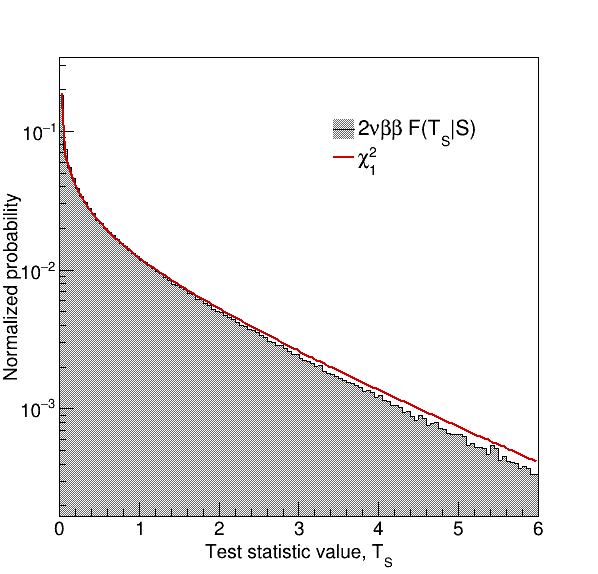
\includegraphics[width=0.33\textwidth]{plots/2nbb-ana/2nbb_teststat.png}%
  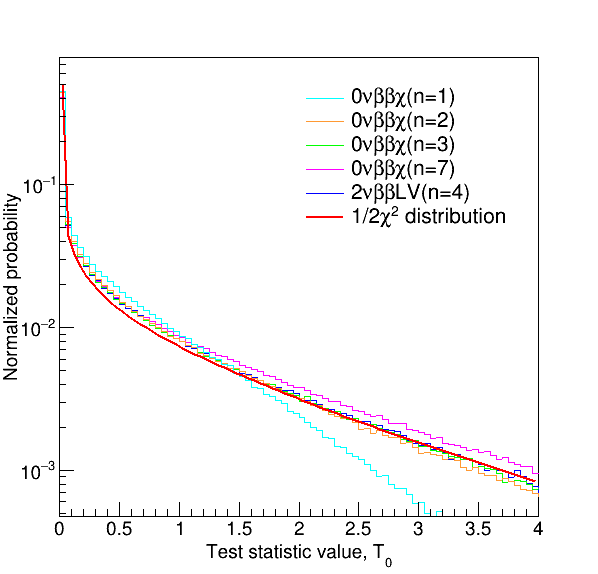
\includegraphics[width=0.33\textwidth]{plots/2nbb-ana/teststatNewphysics.png}%
  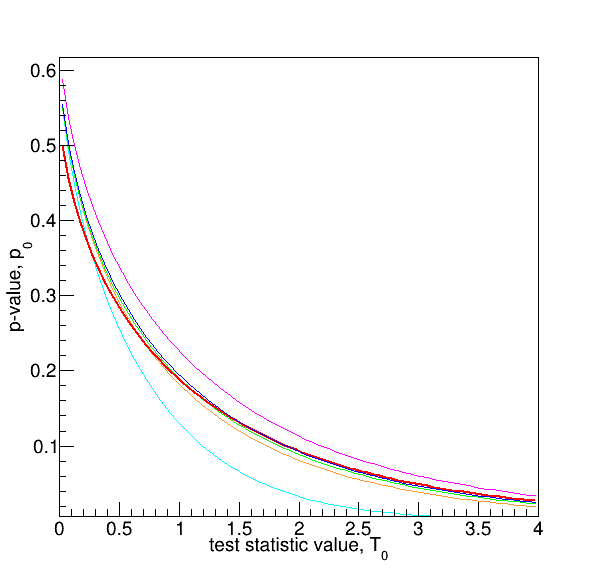
\includegraphics[width=0.33\textwidth]{plots/2nbb-ana/pvalueNewphysics.png}
  \caption{%
    Distribution of the test statistic for various signal hypothesis sampled with Monte
    Carlo methods. The \pvalue\ as a function of the test statistic value, used to extract
    experimental limits on the signals, is shown in the rightmost panel. \fillme{Update}
  }\label{fig:2nbb-ana:ts-dist}
\end{figure}

\blocktitle{sensitivity \\ studies}
The sensitivity to alternative signal hypotheses can be characterized by the median
significance, assuming data generated according to the zero-signal (null) hypothesis, with
which one rejects the signal hypothesis~\cite{Cowan2011}. To compute the sensitivity the
distributions $f(t_S|S)$ and $f(t_S|0)$ are needed. For a discrete set of hypothesis on
the signal $S$, the two distributions are obtained with Toy Monte Carlo and the median
\pvalue\ assuming the null hypothesis is computed. In \cref{fig:2nbb-ana:ts-dist} the median
\pvalue\ as a function of $S$, for all the considered processes is plotted. The sensitivity for 90\%
C.L.~limit setting corresponds to the value of $S$ for which the median \pvalue\ is $0.1$.
In \cref{tab:2nbb-ana:sensitivity} the sensitivities to the half-lives of the investigated
processes are reported.

\blocktitle{fit range \\ and \\ binning}
The fit range is chosen with the purpose of maximizing the signal-to-background ratio and
the signal sensitivity. It starts from the \Arl\ Q-value at 565~keV and stops at the
\nnbb\ Q-value (2039~keV). The \Arl\ background, as a matter of fact, is still dominant
after the LAr veto cut and reduces the signal-to-background ratio to less than 1 in its
energy domain. On the other hand, extending the fit range above the \nnbb\ Q-value does
not improve the signal sensitivity.
\newpar
A 5~keV binning, given the energy resolution of the \enrBEGeII\ data set, does not
remove physical features in the spectrum and is large enough to avoid effects due to
energy scale-related systematic uncertainties. Different bin sizes are tested
to check that the performance of the fit is not affected by this choice.

\begin{table}
  \centering
  \caption{%
    Statistical-only sensitivity for 90\% C.L.~limit setting on the half-lives of some new
    physics processes contributing to the \nnbb\ event distribution. The results are
    extracted from toy Monte Carlo data sets. \fillme{numbers}
  }\label{tab:2nbb-ana:sensitivity}
  \begin{tabular}{lcc}
    \toprule
    Decay                  & Spectral    & Sensitivity     \\
    Mode                   & index ($n$) & (\powtenyr{23}) \\
    \midrule
    \onbbx\                & 1           & \fillme{?}      \\
    \onbbx\                & 2           & \fillme{?}      \\
    $\onbbM\upchi(\upchi)$ & 3           & \fillme{?}      \\
    \onbbxx\               & 7           & \fillme{?}      \\
    \nnbblv\               & 4           & \fillme{?}      \\
    \bottomrule
  \end{tabular}
\end{table}

\section{Systematic uncertainties}%
\label{sec:2nbb-ana:systematics}

Besides the purely-statistical effects, a set of uncertainties which might contribute
systematically to the final analysis uncertainty (both for the \nnbb\ half-life and
new-physics limits) must be considered. Until now, the test statistics studies have been
considering only the effect of Poisson fluctuations in the bin contents, as the generative
model for the toy data sets was fixed. A way to include systematic model uncertainties
when sampling the test statistic distribution is to sample the generative pdf from a set
of `alternative' models according to a certain probability distribution. This is
conceptually equivalent to fitting the data with `wrong' models that assume the presence
of a systematic distortion of the best model. As instance, alternative transition layer
or LAr veto models induce coherent distortions in all background and signal pdfs, which
must be taken into account when generating the toy data sets.
\newpar
This way of treating systematic uncertainties is formalized as a \emph{hybrid
Bayesian-frequentist} approach~\cite{Zyla2020}. In this setting, the distribution
of the test statistic becomes:
\[
  f(t_s) = \int f(t_s | S, \vec{B}, \nu) \pi(\vec{\nu}) d\vec{\nu} \;,
\]
Where $\vec{\nu}$ are the parameters representing the sources of systematic uncertainties
in the model and $\pi(\vec{\nu})$ a `prior' distribution from which $\vec{\nu}$ is sampled
from. The effect introduced by these additional parameters is to smear $f(t_S)$ and
enlarge its tail, weakening the new-physics experimental limits extracted from it. The
software that implements this approach for the \nnbb\ analysis is implemented in the
\texttt{gerda-factor} suite, publicly available on GitHub\footnote{%
  The \texttt{gerda-factory} software suite, available at
  \url{https://github.com/gipert/gerda-factory}, Is implemented in C++ and externally
  depends only on the ROOT libraries for the histogram utilities. The program input is
  specified in JSON format. First, a reference model (in the form of a linear combination
  of histograms, i.e.~the signal pdf, the background pdfs etc.) is set, then the program
  is fed with alternative pdf shapes (histograms) for each of the model components. These
  are grouped according to the source of systematic uncertainty they represent: they can
  be provided for all components at the same time (global distortions) or for selected
  pdfs (specific distortions). The program then computes and stores distortion curves
  ($\text{pdf}_\text{orig}/\text{pdf}_\text{dist}$) for each alternative pdf shape. At run
  time, a distortion curve is randomly selected from each group and applied to the
  reference model; a random data set is then drawn from the obtained model. The procedure
  is repeated in order to generate the required number of randomly-distorted synthetic
  data sets. Optionally, as the alternative pdf shapes are discrete, the program can be
  instructed to consider intermediate distortion curves by interpolation.
}. In the following, the main sources of systematic uncertainties impacting the \nnbb\
analysis are discussed.

\begin{figure}
  \centering
  \includegraphics{plots/2nbb-ana/bege-pdf-dist.pdf}
  \caption{%
    Effect of alternative LAr veto models (right) and transition layer models (left) on
    \kvn\ (signal and high-voltage cables), \kvz\ (homogeneous in the LAr) and \nnbb\
    pdfs for the \enrBEGeII\ data set after the LAr veto cut. See text for details on how
    the alternative models have been constructed.
  }\label{fig:2nbb-ana:pdf-dist}
\end{figure}

\begin{description}[wide]

  \item[LAr veto model] The Monte Carlo LAr veto model, as shown in detail in
    \cref{sec:bkg:lar:ph2:pdfs}, suffers from many uncertainties, some of them arising
    directly from the poor knowledge of LAr channel efficiencies and material optical
    properties implemented in \mage\ (c.f.r~\cref{sec:apdx:mage-optics}). The systematic
    effect of variations of some of these Monte Carlo parameters (i.e.~the LAr absorption
    length, the germanium reflectivity, the coverage of the fiber shroud and the TPB
    quantum efficiency) has been already studied in selected regions of the LAr
    probability map (the object in which the LAr veto model is encoded) in
    \cref{sec:bkg:lar:ph2:heatmap,fig:bkg:lar:ph2:larmap:dist}. Special calibration data
    can be used to determine the channel efficiencies (\cref{sec:bkg:lar:ph2:pcalib}), but
    could not be exploited to reliably constrain other Monte Carlo parameters. This second
    possibility, which requires a much more complex analysis and a deeper understanding of
    simulated and physics data, is discussed in~\cite{Wiesinger2021}.
    \newpar
    To include the LAr veto model uncertainties in the \nnbb\ distribution analysis, the
    following approach has been formulated. First, the special calibration data is
    compared to Monte Carlo simulations to extract three effective channel efficiencies:
    one for all top PMTs, one for all SiPM modules and one for all bottom PMTs
    (\cref{eq:bkg:lar:ph2:chan-eff}). Considering the cylindrical symmetry of the problem
    (a set of detectors arranged in a cylindrical array), A more detailed knowledge of
    efficiencies for each single channel is not necessary. In this reference probability
    map the other Monte Carlo optical parameters are fixed to the values that better
    reflect our degree of belief, which are documented in \cref{sec:apdx:mage-optics}.
    \newpar
    The second step is to provide alternative LAr veto maps for the determination of the
    test statistic distribution, generated with different assumptions for the optical
    parameters. These alternative maps will still have to reproduce the special
    calibration data (i.e.~they will have to be re-tuned on them), which is, technically
    speaking, the \emph{control sample}, but they will differ from the original map in all
    other LAr regions, in particular those probed by the background source simulations.
    Unfortunately, the map generation process is exceptionally expensive from
    the computational point of view (the required time is on the order of several
    thousands of CPU hours), therefore obtaining several alternative probability maps from
    scratch is not feasible. To overcome with this issue, the possibility to perform
    manual distortions of the reference probability map has been investigated.
    \newpar
    An alternative presentation of the probability map distortions in
    \cref{fig:bkg:lar:ph2:larmap:dist}, in which the detection probability in the first
    calibration source position area is set to unity, is given in
    \cref{fig:2nbb-ana:dist-pcanorm} for the germanium reflectivity, the fiber shroud
    coverage and the LAr absorption length (first three panels from left). In this way the
    constraint of reproducing the special calibration data set is made visually explicit,
    as the corresponding probability (in red) is invariant under transformations of the
    Monte Carlo parameters. TPB quantum efficiency and LAr light yield distortions are not
    considered because they can be well-approximated with a global scaling of the
    probability map (i.e.~their effect is fully absorbed in the LAr channel efficiencies).
    The distortions shown in the rightmost panel are obtained in a different way: instead
    of running the full simulation chain with different Monte Carlo parameters to compute
    the detection probability in the selected spatial points, the probability map is
    directly distorted by means of an analytical transformation. A power-law
    transformation is used:
    \begin{equation}\label{eq:2nbb-ana:powerlaw}
      p_k \rightarrow c \cdot p_k^a \;,
    \end{equation}
    in which $p_k$ is the probability value in the LAr voxel $k$ (i.e.~the probability
    map) and $a$ is an arbitrary coefficient controlling the magnitude of the distortion
    and $c$ is a global normalization factor. The latter depends on $a$ and has to be
    adjusted in order to reproduce the total LAr veto event suppression observed in the
    special calibration data. In this sense, the volume of LAr probed by the calibration
    data is a fixed point of the transformation in \cref{eq:2nbb-ana:powerlaw}, and the
    magnitude of the distortion in all other regions is regulated by $a$.
    \newpar
    As it can be stated from \cref{fig:2nbb-ana:dist-pcanorm}, the power-law distortions
    shown in the rightmost panel are not radically different from e.g.~those generated by
    the germanium reflectivity. Moreover, the latter is arguably the most important source
    of systematics in the \nnbb\ analysis, since it probes the LAr volume enclosed by the
    detectors. The power-law map distortion has been therefore judged representative
    enough of the class of distortions generated by fundamental Monte Carlo
    parameters\footnote{%
      It is not difficult to realize that probability map distortions generated by
      fundamental Monte Carlo properties cannot be generally reproduced by global map
      transformations. The effect of these parameters is indeed predominantly local: the
      germanium reflectivity will affect the array region, the fiber shroud coverage the
      region close to the shroud etc. Also the LAr absorption length effect might be
      localized, depending on the scintillation photon mean free path in a certain LAr
      region.  Based on this observation, more complex direct distortions of the map
      limited to certain locations could be also considered. Nevertheless, given the
      expected low impact of LAr veto model uncertainties on the \nnbb\ analysis, this
      option has not been explored.
    }.
    \newpar
    A set of alternative background pdf shapes has been generated with power-law distorted
    maps, varying $a$ from 0.5 to 1.5 in steps of 0.1. The effects on the energy
    spectra of \kvn\ on cables and \kvz\ in LAr have been reported in
    \cref{fig:2nbb-ana:pdf-dist} (left panel), as an example. As it is clear, the
    distortion strongly depends on the energy and the type (Compton scattering, full
    absorption) of the event. All these alternative pdfs have been considered in the
    determination of the distribution of the test statistics, with a flat prior. The
    contribution of LAr veto model uncertainty to the total count is \fillme{?}\%.

    \begin{figure}
      \centering
      \includegraphics{plots/2nbb-ana/larmap-dist-pcanorm.pdf}
      \caption{%
        Study of the impact of Monte Carlo parameters on LAr light detection probabilities in
        various spatial points, normalized to unity at the best value and such to leave the
        probability at the uppermost calibration source position (red point) unchanged. In
        the rightmost panel the effect of a direct, power-law transformation of the
        probability map is shown (no normalization to the red point applied, see text for
        details). The color code and other details are described in
        \cref{fig:bkg:lar:ph2:larmap:dist}.
      }\label{fig:2nbb-ana:dist-pcanorm}
    \end{figure}

  \item[\gesix\ active exposure] The detector fully-active volume (defined
    as the germanium volume in which the charge-collection efficiency reaches unity) and
    enrichment fraction has been estimated for \bege\ detectors up to a certain accuracy
    during a dedicated characterization campaign~\cite{Agostini2015e, Agostini2019}. The
    enriched active volume determines the total amount of detected \nnbb\ counts, and it
    is therefore not expected to produce distortions in the shape of the pdfs. Its effect
    enters in the conversion of the number of signal counts to the corresponding process
    half-life, so this systematic uncertainty component can be included by statistical
    re-sampling the test statistic distribution, while expressing it in units of
    half-life.
    \newpar
    Since three independent estimates of the \bege\ enrichment fraction are
    available\cite{Agostini2015e}, they are combined into the final estimate of 0.880(13)
    by evaluating their variance (see \cref{tab:gerda:efficiencies}). The estimate of the
    full charge-collection depth for each detector required a careful analysis of the
    detector characterization data and is reviewed in
    \cref{apdx:gedetav}~\cite{Agostini2019, Lehnert2016}. The uncertainty on the full
    charge-collection depth estimates is statistically propagated to the active exposure
    by coherently treating the correlated and un-correlated uncertainties. In summary, the
    final estimate of the \enrBEGeII\ data set exposure is
    \[
      \expoM_{76}^\text{AV} = (? \pm ?)~\text{\kgyr} \;.
    \]
    Being the uncertainty of about 1.8\% and considering that it propagates directly
    to the final half-life estimate, the \gesix\ active exposure estimation is the major
    source of systematic uncertainty in the \nnbb\ analysis.

  \item[Transition layer model] As already discussed in several occasions (see in
    particular \cref{apdx:gedetav}), the transition region from the \nplus\ electrode to
    the fully-active detector volume is not completely dead (i.e.~the charge-collection
    efficiency is not zero). Since events interacting with this special region are
    reconstructed with a smaller effective energy, an effect on the energy distribution of
    is expected. Distortions induced by variations of the size of the transition layer are
    particularly noticeable in the \Arl\ event distribution
    (\cref{fig:gedetav:ar39:distortions}) and in the lower tail of intense \g\ peaks
    (\cref{fig:gedetav:calib-optim-example}). A first estimate of the size of the
    transition region for \bege{}s has been extracted from detector characterization
    data~\cite{Lehnert2016}, using a simplified linear model for the charge-collection
    efficiency profile (\cref{fig:gedetav:tl-model}). This estimate, however, has been
    obtained before a significant amount of storage time at room temperature (2--3 years
    before deployment in LAr), in which \nplus\ Lithium profile growing effects took
    place. The effect of this dead-layer growing process on the size of the transition
    region is unfortunately unknown. The assumption of a fixed proportion between the size
    of the transition region and the size of the dead region during the growing process
    leads to results which are clearly incompatible with experimental data (see
    e.g.~\cref{fig:gedetav:calib-optim-example} and \cref{fig:gedetav:ar39-results}).
    \newpar
    To provide a more reliable \bege\ detector transition layer model for the \nnbb\
    analysis, an independent analysis of the \Th\ FEP lower tail from calibration data has
    been performed and documented in detail in \cref{sec:gedetav:calib-optim}. A best-fit
    value of the dead-layer fraction with statistical uncertainty has been obtained for
    each detector. Pdfs for signal and background sources corresponding to the best-fit
    values $\pm1\sigma$, $\pm2\sigma$ and $\pm5\sigma$ ($\sigma$ denotes the statistical
    uncertainty) have been produced and reported in \cref{fig:2nbb-ana:pdf-dist} (right
    panel) for \kvn, \kvz\ and \nnbb\ in the \enrBEGeII\ data set. The pdf distortions are
    noticeably lower than those induced by the LAr veto model uncertainties, and
    contribute with less than 1\% to the total \thalftwo\ systematic uncertainty count.

  \item[Background model] The uncertainty on the location of the main background sources
    is treated as a systematic uncertainty source in the analysis. Pdfs for the same
    radioactive contamination in different locations are provided as an alternative to the
    reference model pdf. In the following table the alternative locations selected for the
    evaluation of the systematic contribution are listed for each fit model component (the
    reference location in \emph{italic}):
    \begin{center}
      \begin{tabular}{ll}
        % \toprule
        Component      & Location                                      \\
        \midrule
        \kvn\ (close)  & \emph{mini-shrouds}, cabling, holder mounting \\
        \kvn\ (far)    & \emph{front-end electronics}, copper shroud   \\
        \kvz\ (close)  & \emph{\nplus\ contact}, \pplus\ contact       \\
        \kvz\ (far)    & \emph{homogeneous in LAr}, above the array    \\
        \Ac\           & \emph{holder mounting}, fiber shroud          \\
        \Bil\ + \Tl\   & \emph{cabling}, outer fibers                  \\
        % \bottomrule
      \end{tabular}
    \end{center}
    Some of these pdfs are shown in \cref{fig:bkg:lar:ph2:pdfs:gmodel}. The contribution
    of background modeling-related uncertainties to the total count amounts to
    \fillme{?}\%.

  \item[Theoretical \nnbb\ decay model] The theoretical calculations of the \nnbb\
    distribution shape are not exact and are based on approximations and assumptions
    (\cref{chap:theory}).  \nnbb\ primary vertices are generated in \mage\ through the
    \decayzero\ program, whose theoretical formulae are documented
    in~\cite{Ponkratenko2000} and references therein. In similar works in the
    past~\cite{Agostini2015a, Agostini2013c} the systematic uncertainty contribution
    arising from the decay theoretical description has been evaluated by considering the
    \nnbb\ distribution obtained with the Primakoff-Rosen
    approximation~\cite{Primakoff1959} as an alternative. The comparison resulted in a
    <1\% effect\footnote{%
      There is, however, no guarantee that the impact on the current analysis is at the
      same, second-order, level. The lower background and higher statistics compared to
      the \phaseone\ data set makes a re-evaluation of this systematic contribution
      necessary. Calculations in the Primakoff-Rosen approximation are known to yield
      results which are more inexact than other (i.e.~those implemented in \decayzero).
      Results from recent calculations (e.g.~phase space factors calculated with exact
      Dirac wave functions with finite nuclear size and electron screening
      effects~\cite{Kotila2012}) are more suitable to this comparison.
      Another source of theoretical uncertainty which has recently turned out to be
      relevant~\cite{Arnold2019, Azzolini2019a} is the assumption on the nuclear state
      configuration of the intermediate nucleus in the decay (\nuc{As}{76} for \nnbb\
      decay of \gesix). In \gesix\ a higher-state dominance (HSD) is usually assumed, but
      a single-state dominance (SSD) cannot be excluded. We are in contact with
      theoreticians to test these different calculation models against the \nnbb\
      distribution collected by \gerda.
    }.

  \item[\mage\ and \geant{}] Another possible source of systematic biases in the analysis
    is the implementation of the experimental setup into the Monte Carlo software stack
    (\mage) and the implementation of the physics processes (particle generation and
    propagation) in \geant. Starting from the first point, uncertainties in the dimension
    and position of the implemented setup components are potentially present in \mage, and
    could in principle affect the shape of the signal and background pdfs. Because of the
    point-like topology of the \nnbb\ decay and uniformity of the \gesix\ isotopic
    fraction, its pdf is expected to depend on the total detector volume and active volume
    model, rather than the exact dimensions or location. The effect of this type of
    uncertainty source has been already investigated above. On the other hand, the shape
    of the background pdfs is expected to depend more on the details of the geometrical
    implementation. This kind of effect, however, is partly similar to (and certainly less
    intense than) the one produced by background model-related uncertainties (see above).
    Moreover, given the modest size of the background sample, it is expected to contribute
    with less than 1\%.
    \newpar
    \geant{} is a broadly-used and heavily-tested software suite in the high-energy
    physics community. No systematic biases due to the implementation of particle creation
    and propagation routines in the code are expected, however there could be some
    originating from uncertainties in the experimental data on which \geant\ relies on
    (i.e.~cross sections and decay widths). To test this eventuality, the full simulation
    chain has been re-run with different electromagnetic low-energy process models
    available in \geant\ (\texttt{Livermore} is the default, alternatives are
    \texttt{Penelope} and \texttt{Standard\_opt3}). The pdfs are observed to change at the
    sub-percent level, and the associated contribution to the systematic uncertainty is
    negligible\footnote{%
      In support of this conclusion, the reader is referred to the official \geant\
      validation portal at \url{https://geant-val.cern.ch} that shows how precise the
      software is in reproducing the experimental cross-section data. \fillme{more on this}
    }.

  \item[Other sources] The energy scale and resolution is another potential source of
    bias in the analysis. Given, however, the excellent resolution of germanium detectors
    and the remarkably precise knowledge of the energy calibration parameters (see
    e.g.~\cref{fig:gerda:calib-desc}), this contribution is negligible. The uncertainty on
    the electron containment, including the one due to uncertainties on the size of the
    detector transition region, and LAr veto efficiency $\epsilon$ in \cref{eq:2nbb:halflife}
    is also negligible.

\end{description}

\begin{table}
  \centering
  \caption{%
    Summary of the systematic uncertainties affecting the \nnbb\ distribution analysis.
    \fillme{numbers}
  }\label{tab:2nbb-ana:systematics}
  \addfontfeatures{Numbers=Tabular}
\begin{tabular}{lcc}
  \toprule
  \mr{2}{Source}              & \mc{2}{Uncertainty}                                       \\
                              & \thalftwo\ (\%)        & \thalfmajo\ 90\% C.L.~limit (\%) \\
  \midrule
  \gesix\ active exposure     & 2.03                   & --                               \\
  LAr veto model              & 0.27                   & --                               \\
  HPGe Transition layer model & $<0.01$                & --                               \\
  Background model            & 0.48                   & --                               \\
  Theoretical \nnbb\ model    & $<0.1$                 & --                               \\
  \mage\ and \geant\          & $<0.1$                 & --                               \\
  \midrule
  Total                       & 2.1                    & --                               \\
  \bottomrule
\end{tabular}

\end{table}

\section{Results and discussion}%
\label{sec:2nbb-ana:results}

Once the analysis procedure has been fixed and the distribution of the test statistic is
determined, its value is computed on real data to extract the \nnbb\ half-life and 90\%
C.L.~lower limits for new-physics processes.

The estimate of the standard \nnbb-decay half-life is
\[
  \thalftwoM = (2.0 \pm \stat{0.0} \pm \syst{0.0}) \cdot 10^{21}~\text{yr} \;.
\]
The statistical and systematic uncertainty is remarkably reduced compared to previous
works~\cite{Agostini2015a}.
\newpar
Lower limits (90\% C.L.) on the half-lives of various Majoron-emitting modes of \onbb\ are
reported in \cref{tab:2nbb-ana:onbbx:limits}. Using phase space factors
from~\cite{Kotila2015} and the most recent set of nuclear matrix elements (the same as the
standard \onbb-decay for spectral index $n=1$, \cite{Hirsch1995} for all the others) it is
possible to convert the half-life limit into a lower limit on the coupling constant \ga.
\newpar
The obtained lower limit on the Lorentz- (and CPT-) violating double-beta decay mode is
\[
  \thalflvM > 0.0 \cdot 10^{23}~\text{yr} \;,
\]
which can be converted into a lower limit on the \aof\ coefficient using phase space
factors in~\cite{Nitescu2020}:
\[
  \aofM > 0 \cdot 10^{-5}~\text{GeV} \;.
\]

\fillme{more comments, compare with previous estimates}

\begin{table}
  \centering
  \caption{%
    90\% C.L.~lower limits for new physics processes contributing to the \nnbb\ event
    distribution. Nuclear matrix elements for $n=1$ are the same as the standard \onbb,
    and have been therefore selected from the most recent nuclear calculations. Matrix
    elements for the other decay modes have been taken from~\cite{Hirsch1995}. Phase space
    factors have been taken from~\cite{Kotila2015}. \fillme{numbers}
  }\label{tab:2nbb-ana:onbbx:limits}
  \addfontfeatures{Numbers=Tabular}
\newcommand{\mrr}[2]{\multirow{#1}[1]{*}{#2}}
\newcommand{\mrc}[2]{\multirowcell{#1}{#2}}

\begin{tabular}{rllccrl}
  \toprule
                     &          &     &               & ($10^{-18}~\text{yr}^{-1}$)          & \mc{2}{90\% C.L.~limit} \\
  \cmidrule(lr){6-7}
  Model              & Mode     & $n$ & \nmemajo\     & \psfmajo\ & $T_{1/2}$ (\powtenyr{23})  & \ga\      \\
  \midrule
  IB                 & \onbbx\  & 1   & 2.66--6.04    & 44.2      & \fillme{?}                 & \fillme{?}      \\
  IC                 & \onbbx\  & 1   & 2.66--6.04    & 44.2      & \fillme{?}                 & \fillme{?}      \\
  ID                 & \onbbxx\ & 3   & $10^{-3\pm1}$ & 0.22      & \fillme{?}                 & \fillme{?}      \\
  IE                 & \onbbxx\ & 3   & $10^{-3\pm1}$ & 0.22      & \fillme{?}                 & \fillme{?}      \\
  IF (bulk)          & \onbbx\  & 2   & {--}          & {--}      & {--}                       & {--}            \\
  \midrule
  IIB                & \onbbx\  & 1   & 2.66--6.04    & 44.2      & \fillme{?}                 & \fillme{?}      \\
  IIC                & \onbbx\  & 3   & 0.16          & 0.073     & \fillme{?}                 & \fillme{?}      \\
  IID                & \onbbxx\ & 3   & $10^{-3\pm1}$ & 0.22      & \fillme{?}                 & \fillme{?}      \\
  IIE                & \onbbxx\ & 7   & $10^{-3\pm1}$ & 0.42      & \fillme{?}                 & \fillme{?}      \\
  IIF                & \onbbx\  & 3   & 0.16          & 0.073     & \fillme{?}                 & \fillme{?}      \\
  \bottomrule
\end{tabular}

\end{table}

\chapsummary
\begin{itemize}
  \item The development of a Monte Carlo model of the \gerda\ LAr veto system (described
    in \cref{chap:bkg:lar:ph2}) makes it possible to obtain predictions on the
    distribution of background and \nnbb\ events in the energy spectrum of data after the
    LAr veto cut. The high statistics of the \nnbb\ data sample ($\sim$$5 \cdot 10^4$
    events in \bege\ detectors above the \Arl\ Q-value from the first part of \phasetwo)
    and the excellent signal-to-background ratio after the LAr veto cut ($\sim$20, a
    factor $\sim$10 better than before the cut) motivates a high-precision analysis of its
    distribution to extract the \nnbb\ half-life and constrain the existence of
    new-physics phenomena (see \cref{chap:theory}).
  \item The data from \bege\ detectors from the first \gexpophasetwobkg\ of \phasetwo\
    is analyzed with a hybrid Bayesian-frequentist approach. Data from semi-coaxial
    detectors is discarded due to the large active volume uncertainties. A test statistic
    based on the profile likelihood ratio is defined, and its distribution with respect to
    the considered (new-)physics signal is studied with Monte Carlo methods. The analysis
    is optimized in order to maximize the sensitivity for limit setting to new-physics
    signals. Sensitivities to Majoron-emitting \onbb\ modes or Lorentz-violating \nnbb\
    are obtained in the $10^{23}$--$10^{24}$~yr.
  \item Various sources of systematic uncertainties are considered in the computation of
    the test statistic distribution by introducing distortions of the reference model of
    the Monte Carlo toy data sets. Various alternative LAr veto models and detector
    transition layer models are used to produce the background and signal pdfs, but their
    effect on the test statistic distribution is of the order of 1\% or less. The main
    source of systematic uncertainty remains the detector active volume estimation, which
    contributes with \fillme{?}\% to the total uncertainty count.
  \item Final results for \thalftwo\ \fillme{\ldots}
\end{itemize}

% vim: tw=90
